% Created 2020-10-12 Mon 13:23
% Intended LaTeX compiler: pdflatex
\documentclass[11pt]{article}
\usepackage[utf8]{inputenc}
\usepackage[T1]{fontenc}
\usepackage{graphicx}
\usepackage{grffile}
\usepackage{longtable}
\usepackage{wrapfig}
\usepackage{rotating}
\usepackage[normalem]{ulem}
\usepackage{amsmath}
\usepackage{textcomp}
\usepackage{amssymb}
\usepackage{capt-of}
\usepackage[hidelinks]{hyperref}
\usepackage{minted}
\usepackage[a4paper, total={6in, 9in}]{geometry}
\setminted{breaklines, autogobble}
\usemintedstyle{emacs}
\author{Nebhrajani A. V.}
\date{}
\title{Python IP Class Notebook}
\hypersetup{
 pdfauthor={Nebhrajani A. V.},
 pdftitle={Python IP Class Notebook},
 pdfkeywords={},
 pdfsubject={},
 pdfcreator={Emacs 25.2.2 (Org mode 9.3.6)},
 pdflang={English}}
\begin{document}

\maketitle
\tableofcontents

\newpage

\section{Preamble}
\label{sec:org12c86df}
\subsection{Notebook Conventions}
\label{sec:org951c2bd}
All code in this notebook is in Python unless specified otherwise.
All code is syntax-highlighted, placed in boxes, and is line
numbered. The output of the interpreter on \texttt{stdout} is printed directly below it,
\texttt{verbatim}, thus.
\begin{minted}[,frame=single, framesep=10pt, linenos]{python}
# Print Hello world!
print("Hello world!")
\end{minted}

\begin{verbatim}
Hello world!
\end{verbatim}


It is recommended that you navigate using the hyperlinked TOC or the Adobe
Bookmarks tree.

\subsection{Hardware and Software Used}
\label{sec:orgf141c26}

 This notebook is written in an \texttt{org-mode} file and exported to PDF via \LaTeX{}, Org version 9.3.6 on
GNU Emacs 25.2.2 (x86\_ 64-pc-linux-gnu, GTK+ Version 3.22.21) of
2017-09-23, modified by Debian, on a Foxconn Core i7 NanoPC running Linux
Mint 19.3 XFCE 64-bit. Python 2.7.17 of 2020-04-15 is used
throughout unless specified otherwise. For the Org or \LaTeX{} source, contact
\href{mailto:aditya.v.nebhrajani@gmail.com}{aditya.v.nebhrajani@gmail.com}.

\subsection{Acknowledgements}
\label{sec:org14a8b5f}
I am grateful to the FSF, the GNU Project, the Linux foundation,
the Emacs, StackExchange and FLOSS communities, and my father,
who taught me that a world outside commercialized technology does
exist and thrive.
\newpage

\section{NumPy}
\label{sec:org70f8fdf}
\subsection{Worksheet 2020-07-26}
\label{sec:org39c9d1a}

\begin{enumerate}
\item Create an ndarray with values ranging from 10 to 49 each spaced with a difference of 3.
\begin{minted}[,frame=single, framesep=10pt, linenos]{python}
import numpy as np
arr=np.arange(10,50,3,dtype=int)
print(arr)
\end{minted}

\begin{verbatim}
[10 13 16 19 22 25 28 31 34 37 40 43 46 49]
\end{verbatim}

\item Find the output of the following Python code:

\begin{minted}[,frame=single, framesep=10pt, linenos]{python}
x="hello world"
print(x[:2],x[:-2],x[-2:])
\end{minted}

\begin{verbatim}
he hello wor ld
\end{verbatim}

\item Predict the output of the following code fragments:

\begin{minted}[,frame=single, framesep=10pt, linenos]{python}
import numpy as np
x=np.array([1,2,3])
y=np.array([3,2,1])
z=np.concatenate([x,y])
print(z)
\end{minted}

\begin{verbatim}
[1 2 3 3 2 1]
\end{verbatim}

\item Consider following two arrays: Array1=
array([0,1,2],[3,4,5],[6,7,8]]) and Array2=
array([10,11,12],[13,14,15],[16,17,18]]). Write NumPy command to concatenate Array1 and Array2:

\begin{enumerate}
\item Row wise
\begin{minted}[,frame=single, framesep=10pt, linenos]{python}
import numpy as np
Array1= np.array([[0,1,2],[3,4,5],[6,7,8]])
Array2= np.array([[10,11,12],[13,14,15],[16,17,18]])
rarr=np.concatenate([Array1,Array2],axis=1)
print(rarr)
\end{minted}

\begin{verbatim}
[[ 0  1  2 10 11 12]
 [ 3  4  5 13 14 15]
 [ 6  7  8 16 17 18]]
\end{verbatim}

\item Column wise
\begin{minted}[,frame=single, framesep=10pt, linenos]{python}
import numpy as np
Array1= np.array([[0,1,2],[3,4,5],[6,7,8]])
Array2= np.array([[10,11,12],[13,14,15],[16,17,18]])
carr=np.concatenate([Array1,Array2],axis=0)
print(carr)
\end{minted}

\begin{verbatim}
[[ 0  1  2]
 [ 3  4  5]
 [ 6  7  8]
 [10 11 12]
 [13 14 15]
 [16 17 18]]
\end{verbatim}
\end{enumerate}

\item To create sequences of numbers, NumPy provides a function \uline{(a)arange} analogous to range that returns arrays instead of lists.

\item Find the output of following program.
\begin{minted}[,frame=single, framesep=10pt, linenos]{python}
import numpy as np
a=np.array([30,60,70,30,10,86,45])
print(a[-2:6])
\end{minted}

\begin{verbatim}
[86]
\end{verbatim}

\item Write a NumPy program to create a 2d array with 1 on the border and 0 inside.
\begin{minted}[,frame=single, framesep=10pt, linenos]{python}
import numpy as np
x = np.ones((5,5))
print("Original array:")
print(x)
print("1 on the border and 0 inside in the array")
x[1:-1,1:-1] = 0
print(x)
\end{minted}

\begin{verbatim}
Original array:
[[1. 1. 1. 1. 1.]
 [1. 1. 1. 1. 1.]
 [1. 1. 1. 1. 1.]
 [1. 1. 1. 1. 1.]
 [1. 1. 1. 1. 1.]]
1 on the border and 0 inside in the array
[[1. 1. 1. 1. 1.]
 [1. 0. 0. 0. 1.]
 [1. 0. 0. 0. 1.]
 [1. 0. 0. 0. 1.]
 [1. 1. 1. 1. 1.]]
\end{verbatim}

\item Given following ndarray A: ([[2, 4, 6], [7, 8, 9], [1, 2, 3]])
Write the python statements to perform the array slices in the
way so as to extract first row and second column.
\begin{minted}[,frame=single, framesep=10pt, linenos]{python}
import numpy as np
A = np.array([[2,4,6],[7,8,9],[1,2,3]])
print(A[0,:])
print(A[:,1])
\end{minted}

\begin{verbatim}
[2 4 6]
[4 8 2]
\end{verbatim}

\item Write python statement to create a two- dimensional array of 4 rows and 3 columns. The array should be filled with ones.
\begin{minted}[,frame=single, framesep=10pt, linenos]{python}
import numpy as np
x = np.ones((4,3))
print(x)
\end{minted}

\begin{verbatim}
[[1. 1. 1.]
 [1. 1. 1.]
 [1. 1. 1.]
 [1. 1. 1.]]
\end{verbatim}

\item Find the output of following program.
\begin{minted}[,frame=single, framesep=10pt, linenos]{python}
import numpy as np
d = np.array([10,20,30,40,50,60,70])
print(d[-5:])
\end{minted}

\begin{verbatim}
[30 40 50 60 70]
\end{verbatim}

\item State at least two differences between a NumPy array and a list
\begin{center}
\begin{tabular}{|l|l|}
\hline
NumPy Array & List\\
\hline
By default, numpy arrays are homogeneous & They can have elements of different data types\\
Element-wise operations are possible & Element-wise operations don’t work on lists\\
They take up less space & They take up more space\\
\hline
\end{tabular}
\end{center}

\item Find the output of following program.
\begin{minted}[,frame=single, framesep=10pt, linenos]{python}
import numpy as np
d=np.array([10,20,30,40,50,60,70])
print(d[-1:-4:-1])
\end{minted}

\begin{verbatim}
[70 60 50]
\end{verbatim}

\item Write the output of the following code.
\begin{minted}[,frame=single, framesep=10pt, linenos]{python}
import numpy as np
a=[[1,2,3,4],[5,6,7,8]]
b=[[1,2,3,4],[5,6,7,8]]
n=np.concatenate((a, b), axis=0)
print(n[1])
print(n[1][1])
\end{minted}

\begin{verbatim}
[5 6 7 8]
6
\end{verbatim}

\item Which of the following is contained in NumPy library?
\begin{enumerate}
\item \textbf{N-Dimensional Array Object}
\item Series
\item DataFrame
\item Plot
\end{enumerate}

\item Point out the correct statement:
\begin{enumerate}
\item NumPy main object is the homogeneous multidimensional array
\item In Numpy, dimensions are called axes
\item NumPy array class is called ndarray
\item \textbf{All of the above}
\end{enumerate}

\item When the fromiter() is preferred over array()?
\textbf{A:} Fromiter() is preferred over array()for creating non-numeric
sequences like strings and dictionaries.

\item What is the purpose of order argument in empty(). What do ‘C’
and ‘F’ stands for? What is the default value of order
argument?
\textbf{A:} The “order” argument arranges the elements of the
array row-wise or column-wise. C order arranges elements column
wise and means “c”-like, whereas F order arranges elements row
wise and means “fortran”-like. Default value of order argument
is C.

\item Differentiate split() from hsplit() and vsplit().
\textbf{A:} Split() function is a general function which can be used to split an
array in numpy both horizontally and vertically by providing an
axis. If the axis is 0 it is the same as hsplit() and if the
axis is 1 it behaves as vsplit(). The difference between
split() and hsplit(),vsplit() is that split() allows you to
specify the axis that you wish, and hsplit() and vsplit() are
for specific axes.

\item Find the output:
\begin{enumerate}
\item \begin{minted}[,frame=single, framesep=10pt, linenos]{python}
import numpy as np
a = np.linspace(2.5,5,6)
print(a)
\end{minted}

\begin{verbatim}
[2.5 3.  3.5 4.  4.5 5. ]
\end{verbatim}

\item \begin{minted}[,frame=single, framesep=10pt, linenos]{python}
import numpy as np
a=np.array([[0,2,4,6],[8,10,12,14],[16,18,20,22],[24,26,28,30]])
print(a)
print(a[:3,3:])
print(a[1::2,:3])
print(a[-3:-1,-4::2])
print(a[::-1,::-1])
\end{minted}

\begin{verbatim}
[[ 0  2  4  6]
 [ 8 10 12 14]
 [16 18 20 22]
 [24 26 28 30]]
[[ 6]
 [14]
 [22]]
[[ 8 10 12]
 [24 26 28]]
[[ 8 12]
 [16 20]]
[[30 28 26 24]
 [22 20 18 16]
 [14 12 10  8]
 [ 6  4  2  0]]
\end{verbatim}
\end{enumerate}
\end{enumerate}

\newpage
\section{Pandas}
\label{sec:orgac8afcf}
\subsection{Series}
\label{sec:org0c2055f}
\begin{minted}[,frame=single, framesep=10pt, linenos]{python}
# Import numpy and pandas
import pandas as pd
import numpy as np

# Create an empty series
s = pd.Series()
print(s)

# Series from ndarray
data = np.array(['a', 'b', 'c', 'd'])

## Without index
s = pd.Series(data)
print(s)
## With index
s = pd.Series(data, index = [100, 101, 102, 103])
print(s)

# Scalar series
s = pd.Series(5, index = [0, 1, 2, 3])
print(s)

# Series from dictionary
data = {'a' : 0., 'b' : 1., 'c' : 2.}

## Without index
s = pd.Series(data)
print(s)
## With index
s = pd.Series(data, index = ['b', 'c', 'd', 'a'])
print(s)

# Another dictionary example
f_dict = {'apples': 500, 'kiwi': 20, 'oranges': 100, 'cherries': 6000}
print(f_dict)

arr = pd.Series(f_dict)
print('\nArray Items')
print(arr)
\end{minted}

\begin{verbatim}
Series([], dtype: float64)
0    a
1    b
2    c
3    d
dtype: object
100    a
101    b
102    c
103    d
dtype: object
0    5
1    5
2    5
3    5
dtype: int64
a    0.0
b    1.0
c    2.0
dtype: float64
b    1.0
c    2.0
d    NaN
a    0.0
dtype: float64
{'apples': 500, 'kiwi': 20, 'oranges': 100, 'cherries': 6000}

Array Items
apples       500
kiwi          20
oranges      100
cherries    6000
dtype: int64
\end{verbatim}

\begin{minted}[,frame=single, framesep=10pt, linenos]{python}
# Indexing
import pandas as pd
from pandas import Series
arr = Series([22, 44, 66, 88, 108])
print(arr[[1, 3, 0, 4]])
\end{minted}

\begin{verbatim}
1     44
3     88
0     22
4    108
dtype: int64
\end{verbatim}


\begin{minted}[,frame=single, framesep=10pt, linenos]{python}
# Series operations
import pandas as pd
ds1 = pd.Series([2, 4, 6, 8, 10])
ds2 = pd.Series([1, 3, 5, 7, 9])
print(ds1)
print(ds2)
ds = ds1 + ds2
print("Add two Series:")
print(ds)
print("Subtract two Series:")
ds = ds1 - ds2
print(ds)
print("Multiply two Series:")
ds = ds1 * ds2
print(ds)
print("Divide Series1 by Series2:")
ds = ds1 / ds2
print(ds)
\end{minted}

\begin{verbatim}
0     2
1     4
2     6
3     8
4    10
dtype: int64
0    1
1    3
2    5
3    7
4    9
dtype: int64
Add two Series:
0     3
1     7
2    11
3    15
4    19
dtype: int64
Subtract two Series:
0    1
1    1
2    1
3    1
4    1
dtype: int64
Multiply two Series:
0     2
1    12
2    30
3    56
4    90
dtype: int64
Divide Series1 by Series2:
0    2.000000
1    1.333333
2    1.200000
3    1.142857
4    1.111111
dtype: float64
\end{verbatim}

\begin{minted}[,frame=single, framesep=10pt, linenos]{python}
# Series to array
import pandas as pd
import numpy as np
s1 = pd.Series(['100', '200', '300', 'python'])
print("Original data series")
print(s1)
print("Series to array")
a = np.array(s1.values.tolist())
print(a)
\end{minted}

\begin{verbatim}
Original data series
0       100
1       200
2       300
3    python
dtype: object
Series to array
['100' '200' '300' 'python']
\end{verbatim}


\begin{minted}[,frame=single, framesep=10pt, linenos]{python}
# Heads and tails
import pandas as pd
import math
s = pd.Series(data = [math.sqrt(x) for x in range(1,10)],
              index = [x for x in range(1,10)])
print(s)
print(s.head(6))
print(s.tail(7))
print(s.head())
print(s.tail())
\end{minted}

\begin{verbatim}
1    1.000000
2    1.414214
3    1.732051
4    2.000000
5    2.236068
6    2.449490
7    2.645751
8    2.828427
9    3.000000
dtype: float64
1    1.000000
2    1.414214
3    1.732051
4    2.000000
5    2.236068
6    2.449490
dtype: float64
3    1.732051
4    2.000000
5    2.236068
6    2.449490
7    2.645751
8    2.828427
9    3.000000
dtype: float64
1    1.000000
2    1.414214
3    1.732051
4    2.000000
5    2.236068
dtype: float64
5    2.236068
6    2.449490
7    2.645751
8    2.828427
9    3.000000
dtype: float64
\end{verbatim}

\begin{minted}[,frame=single, framesep=10pt, linenos]{python}
# Sorting pandas series
import pandas as pd
s = pd.Series(['100', '200', 'python', '300.12', '400'])
print("Original data series:")
print(s)
asc_s = pd.Series(s).sort_values()
print(asc_s)
dsc_s = pd.Series(s).sort_values(ascending=False)
print(dsc_s)

# Appending
new_s = s.append(pd.Series(['500', 'php']))
print(new_s)
\end{minted}

\begin{verbatim}
Original data series:
0       100
1       200
2    python
3    300.12
4       400
dtype: object
0       100
1       200
3    300.12
4       400
2    python
dtype: object
2    python
4       400
3    300.12
1       200
0       100
dtype: object
0       100
1       200
2    python
3    300.12
4       400
0       500
1       php
dtype: object
\end{verbatim}

\begin{minted}[,frame=single, framesep=10pt, linenos]{python}
# Mean and median
import pandas as pd
s = pd.Series(data = [1,2,3,4,5,6,7,8,9,5,3])
print("Original data series:")
print(s)
print("Mean:")
print(s.mean())
print("Standard deviation:")
print(s.std())
\end{minted}

\begin{verbatim}
Original data series:
0     1
1     2
2     3
3     4
4     5
5     6
6     7
7     8
8     9
9     5
10    3
dtype: int64
Mean:
4.818181818181818
Standard deviation:
2.522624895547565
\end{verbatim}

\begin{minted}[,frame=single, framesep=10pt, linenos]{python}
# Isin function
import numpy as np
import pandas as pd

s = pd.Series(['dog', 'cow', 'dog', 'cat', 'lion'], name='animal')

r = s.isin(['dog', 'cat'])
print(r)
\end{minted}

\begin{verbatim}
0     True
1    False
2     True
3     True
4    False
Name: animal, dtype: bool
\end{verbatim}


\begin{minted}[,frame=single, framesep=10pt, linenos]{python}
# Appending and concatenation
 import numpy as np
 import pandas as pd

 # Input
 ser1 = pd.Series(range(5))
 ser2 = pd.Series(list('abcde'))

 # Vertical
 ser3 = ser1.append(ser2)
 print(ser3)

 # Or using Pandas concatenate along axis 0
 ser3 = pd.concat([ser1, ser2], axis = 0)
 print(ser3)

 # Horizontal (into a dataframe)
 ser3 = pd.concat([ser1, ser2], axis = 1)
 print(ser3)
\end{minted}

\subsection{DataFrame}
\label{sec:orge72ba18}

\begin{minted}[,frame=single, framesep=10pt, linenos]{python}
# Empty dataframe
import pandas as pd

data = pd.DataFrame()
print(data)
\end{minted}

\begin{verbatim}
Empty DataFrame
Columns: []
Index: []
\end{verbatim}



\begin{minted}[,frame=single, framesep=10pt, linenos]{python}
# Dataframe from list
import pandas as pd

table = [1, 2, 3, 4, 5]
data = pd.DataFrame(table)
print(data)
\end{minted}

\begin{verbatim}
   0
0  1
1  2
2  3
3  4
4  5
\end{verbatim}


\begin{minted}[,frame=single, framesep=10pt, linenos]{python}
# Dataframe from mixed list
import pandas as pd

table = [[1, 'Nebhrajani'], [2, 'Python'], [3, 'Hello']]
data = pd.DataFrame(table)
print(data)
\end{minted}

\begin{verbatim}
   0           1
0  1  Nebhrajani
1  2      Python
2  3       Hello
\end{verbatim}


\begin{minted}[,frame=single, framesep=10pt, linenos]{python}
# Column labels
import pandas as pd

table = [[1, 'Nebhrajani'], [2, 'Python'], [3, 'Hello']]
data = pd.DataFrame(table, columns = ['S.No', 'Name'])
print(data)
\end{minted}

\begin{verbatim}
   S.No        Name
0     1  Nebhrajani
1     2      Python
2     3       Hello
\end{verbatim}


\begin{minted}[,frame=single, framesep=10pt, linenos]{python}
# Random numbers dataframe
import numpy as np
import pandas as pd

d_frame = pd.DataFrame(np.random.randn(8, 4))
print(d_frame)
\end{minted}

\begin{verbatim}
          0         1         2         3
0  1.229859  0.276771 -0.045632  0.259311
1  0.074277 -0.168431  1.667804 -1.407468
2  0.237926 -0.839273 -0.507893 -1.479707
3 -1.406518  0.925847  1.197716 -1.009840
4 -2.363665 -1.150008  0.667568 -0.633510
5  0.145881  0.369782  0.261877 -0.740075
6  0.807986  1.199728 -0.492667  0.222350
7 -0.043676  0.477135  0.145498  0.965713
\end{verbatim}


\begin{minted}[,frame=single, framesep=10pt, linenos]{python}
# Dataframe from dict
import pandas as pd

table = {'name': ['Aditya', 'Aryan', 'Nebhrajani', 'Sahej'],
        'Salary':[1000000, 1200000, 900000, 1100000]}

data = pd.DataFrame(table)
print(data)
\end{minted}

\begin{verbatim}
         name   Salary
0      Aditya  1000000
1       Aryan  1200000
2  Nebhrajani   900000
3       Sahej  1100000
\end{verbatim}


\begin{minted}[,frame=single, framesep=10pt, linenos]{python}
# Dataframe from some given dictionary data
import pandas as pd
import numpy as np

exam_data  = {'name': ['Anastasia', 'Dima', 'Katherine', 'James',
              'Emily', 'Michael', 'Matthew', 'Laura', 'Kevin', 'Jonas'],
        'score': [12.5, 9, 16.5, np.nan, 9, 20, 14.5, np.nan, 8, 19],
        'attempts': [1, 3, 2, 3, 2, 3, 1, 1, 2, 1],
        'qualify': ['yes', 'no', 'yes', 'no', 'no', 'yes', 'yes',
                    'no', 'no', 'yes']}
labels = ['a', 'b', 'c', 'd', 'e', 'f', 'g', 'h', 'i', 'j']

df = pd.DataFrame(exam_data , index=labels)
print(df)
\end{minted}

\begin{verbatim}
        name  score  attempts qualify
a  Anastasia   12.5         1     yes
b       Dima    9.0         3      no
c  Katherine   16.5         2     yes
d      James    NaN         3      no
e      Emily    9.0         2      no
f    Michael   20.0         3     yes
g    Matthew   14.5         1     yes
h      Laura    NaN         1      no
i      Kevin    8.0         2      no
j      Jonas   19.0         1     yes
\end{verbatim}

\begin{minted}[,frame=single, framesep=10pt, linenos]{python}
# Messing with columns
import pandas as pd

table = {'name': ['Aditya', 'Aryan', 'Nebhrajani', 'Sahej'],
         'Age': [25, 32, 30, 26],
         'Profession': ['Developer', 'Analyst', 'Admin', 'HR'],
         'Salary':[1000000, 1200000, 900000, 1100000]
         }

data1 = pd.DataFrame(table)
print(data1)

print('\n After Changing the Column Order')
data2 = pd.DataFrame(table, columns = ['name', 'Profession', 'Salary',
                                       'Age'])
print(data2)
print('\n Using Wrong Column ')
data3 = pd.DataFrame(table, columns = ['name', 'Qualification', 'Salary',
                                       'Age'])
print(data3)
\end{minted}

\begin{verbatim}
         name  Age Profession   Salary
0      Aditya   25  Developer  1000000
1       Aryan   32    Analyst  1200000
2  Nebhrajani   30      Admin   900000
3       Sahej   26         HR  1100000

 After Changing the Column Order
         name Profession   Salary  Age
0      Aditya  Developer  1000000   25
1       Aryan    Analyst  1200000   32
2  Nebhrajani      Admin   900000   30
3       Sahej         HR  1100000   26

 Using Wrong Column
         name Qualification   Salary  Age
0      Aditya           NaN  1000000   25
1       Aryan           NaN  1200000   32
2  Nebhrajani           NaN   900000   30
3       Sahej           NaN  1100000   26
\end{verbatim}

\begin{minted}[,frame=single, framesep=10pt, linenos]{python}
# Dataframe indexing
import pandas as pd

table = {'name': ['Aditya', 'Aryan', 'Nebhrajani', 'Sahej'],
         'Age': [25, 32, 30, 26],
         'Profession': ['Developer', 'Analyst', 'Admin', 'HR'],
         'Salary':[1000000, 1200000, 900000, 1100000]
         }
data = pd.DataFrame(table)
print(data)

print('\nSetting name as an index')
new_data = data.set_index('name')
print(new_data)

print('\nReturn Index Aditya Details')
print(new_data.loc['Aditya'])
\end{minted}

\begin{verbatim}
         name  Age Profession   Salary
0      Aditya   25  Developer  1000000
1       Aryan   32    Analyst  1200000
2  Nebhrajani   30      Admin   900000
3       Sahej   26         HR  1100000

Setting name as an index
            Age Profession   Salary
name
Aditya       25  Developer  1000000
Aryan        32    Analyst  1200000
Nebhrajani   30      Admin   900000
Sahej        26         HR  1100000

Return Index Aditya Details
Age                  25
Profession    Developer
Salary          1000000
Name: Aditya, dtype: object
\end{verbatim}

\begin{minted}[,frame=single, framesep=10pt, linenos]{python}
# Getting columns
import pandas as pd

table = {'name': ['Aditya', 'Aryan', 'Nebhrajani', 'Sahej'],
         'Age': [25, 31, 35, 26],
         'Salary':[100000, 120000, 700000, 110000]
            }

data = pd.DataFrame(table)
print(data)
print('\nShape and Size of a DataFrame')
print(data.shape)
data2 = pd.DataFrame(table, columns = ['name', 'Profession', 'Salary',
                                       'Age'])
data3 = pd.DataFrame(table, columns = ['name', 'Qualification', 'Salary',
                                       'Age'])
print('Data2 Values ')
print(data2.values)
print('\nData3 Values ')
print(data3.values)
data1 = pd.DataFrame(table)
table = {'Age': [25, 32, 30, 26],
         'Salary':[1000000, 1200000, 900000, 1100000]
         }
data4 = pd.DataFrame(table)
data1.index.name = 'Emp No'
print(data1)
print()
data4.index.name = 'Cust No'
print(data4)
data1.columns.name = 'Employee Details'
print(data1)
data4.columns.name = 'Customers Information'
print(data4)
data1 = pd.DataFrame(table)
print(data1)
print('\nDescribe function result')
print(data1.describe())
\end{minted}

\begin{verbatim}
         name  Age  Salary
0      Aditya   25  100000
1       Aryan   31  120000
2  Nebhrajani   35  700000
3       Sahej   26  110000

Shape and Size of a DataFrame
(4, 3)
Data2 Values
[['Aditya' nan 100000 25]
 ['Aryan' nan 120000 31]
 ['Nebhrajani' nan 700000 35]
 ['Sahej' nan 110000 26]]

Data3 Values
[['Aditya' nan 100000 25]
 ['Aryan' nan 120000 31]
 ['Nebhrajani' nan 700000 35]
 ['Sahej' nan 110000 26]]
              name  Age  Salary
Emp No
0           Aditya   25  100000
1            Aryan   31  120000
2       Nebhrajani   35  700000
3            Sahej   26  110000

         Age   Salary
Cust No
0         25  1000000
1         32  1200000
2         30   900000
3         26  1100000
Employee Details        name  Age  Salary
Emp No
0                     Aditya   25  100000
1                      Aryan   31  120000
2                 Nebhrajani   35  700000
3                      Sahej   26  110000
Customers Information  Age   Salary
Cust No
0                       25  1000000
1                       32  1200000
2                       30   900000
3                       26  1100000
   Age   Salary
0   25  1000000
1   32  1200000
2   30   900000
3   26  1100000

Describe function result
             Age        Salary
count   4.000000  4.000000e+00
mean   28.250000  1.050000e+06
std     3.304038  1.290994e+05
min    25.000000  9.000000e+05
25%    25.750000  9.750000e+05
50%    28.000000  1.050000e+06
75%    30.500000  1.125000e+06
max    32.000000  1.200000e+06
\end{verbatim}

\begin{minted}[,frame=single, framesep=10pt, linenos]{python}
# Getting rows using loc
import pandas as pd
table = {'name': ['Jai', 'Mike', 'Suresh', 'Sahej'],
         'Age': [25, 32, 30, 26],
         'Profession': ['Developer', 'Analyst', 'Admin', 'HR'],
         'Salary':[1000000, 1200000, 900000, 1100000]}

data = pd.DataFrame(table, index = ['a', 'b', 'c', 'd'])
print(data)

print('\n---Select b row from a DataFrame---')
print(data.loc['b'])

print('\n---Select c row from a DataFrame---')
print(data.loc['c'])

print('\n---Select b and d rows from a DataFrame---')
print(data.loc[['b', 'd']])
\end{minted}

\begin{verbatim}
     name  Age Profession   Salary
a     Jai   25  Developer  1000000
b    Mike   32    Analyst  1200000
c  Suresh   30      Admin   900000
d   Sahej   26         HR  1100000

---Select b row from a DataFrame---
name             Mike
Age                32
Profession    Analyst
Salary        1200000
Name: b, dtype: object

---Select c row from a DataFrame---
name          Suresh
Age               30
Profession     Admin
Salary        900000
Name: c, dtype: object

---Select b and d rows from a DataFrame---
    name  Age Profession   Salary
b   Mike   32    Analyst  1200000
d  Sahej   26         HR  1100000
\end{verbatim}

\begin{minted}[,frame=single, framesep=10pt, linenos]{python}
# Getting columns using loc
import pandas as pd
table = {'Name': ['Abhimanyu', 'Jai', 'Suresh', 'Sahej', 'Shail'],
         'Age': [35, 25, 32, 30, 29],
         'Profession': ['Manager', 'Developer', 'Analyst', 'Admin', 'HR'],
         'Sale':[422.19, 22.55, 119.470, 200.190, 44.55],
         'Salary':[12000, 10000, 14000, 11000, 14000]}

data = pd.DataFrame(table)
print(data)

print('\n---Select Name, Sale column in a DataFrame---')
print(data.loc[:, ['Name', 'Sale']])

print('\n---Select Name, Profession, Salary in a DataFrame---')
print(data.loc[:, ['Name', 'Profession', 'Salary']])

print('\n---Select rows from 1 to 2 in a DataFrame---')
print(data.loc[1:3, ['Name', 'Profession', 'Salary']])
\end{minted}

\begin{verbatim}
        Name  Age Profession    Sale  Salary
0  Abhimanyu   35    Manager  422.19   12000
1        Jai   25  Developer   22.55   10000
2     Suresh   32    Analyst  119.47   14000
3      Sahej   30      Admin  200.19   11000
4      Shail   29         HR   44.55   14000

---Select Name, Sale column in a DataFrame---
        Name    Sale
0  Abhimanyu  422.19
1        Jai   22.55
2     Suresh  119.47
3      Sahej  200.19
4      Shail   44.55

---Select Name, Profession, Salary in a DataFrame---
        Name Profession  Salary
0  Abhimanyu    Manager   12000
1        Jai  Developer   10000
2     Suresh    Analyst   14000
3      Sahej      Admin   11000
4      Shail         HR   14000

---Select rows from 1 to 2 in a DataFrame---
     Name Profession  Salary
1     Jai  Developer   10000
2  Suresh    Analyst   14000
3   Sahej      Admin   11000
\end{verbatim}

\begin{minted}[,frame=single, framesep=10pt, linenos]{python}
# Getting rows using iloc
import pandas as pd

table = {'name': ['Jai', 'Mit', 'Suresh', 'Tammanah'],
         'Age': [25, 32, 30, 26],
         'Profession': ['Developer', 'Analyst', 'Admin', 'HR'],
         'Salary':[1000000, 1200000, 900000, 1100000]}
data = pd.DataFrame(table, index = ['a', 'b', 'c', 'd'])
print(data)

print('\n---Select 1st row from a DataFrame---')
print(data.iloc[1])

print('\n---Select 3rd row from a DataFrame---')
print(data.iloc[3])

print('\n---Select 1 and 3 rows from a DataFrame---')
print(data.iloc[[1, 3]])
\end{minted}

\begin{verbatim}
       name  Age Profession   Salary
a       Jai   25  Developer  1000000
b       Mit   32    Analyst  1200000
c    Suresh   30      Admin   900000
d  Tammanah   26         HR  1100000

---Select 1st row from a DataFrame---
name              Mit
Age                32
Profession    Analyst
Salary        1200000
Name: b, dtype: object

---Select 3rd row from a DataFrame---
name          Tammanah
Age                 26
Profession          HR
Salary         1100000
Name: d, dtype: object

---Select 1 and 3 rows from a DataFrame---
       name  Age Profession   Salary
b       Mit   32    Analyst  1200000
d  Tammanah   26         HR  1100000
\end{verbatim}

\begin{minted}[,frame=single, framesep=10pt, linenos]{python}
# Assignment: conditional loc-ing
import pandas as pd
import numpy as np

data = pd.DataFrame({
    'Age' :     [ 10, 22, 13, 21, 12, 11, 17],
    'Section' : [ 'A', 'B', 'C', 'B', 'B', 'A', 'A'],
    'City' :    [ 'Gurgaon', 'Delhi', 'Mumbai', 'Delhi',
                  'Mumbai', 'Delhi', 'Mumbai'],
    'Gender' :  [ 'M', 'F', 'F', 'M', 'M', 'M', 'F'],
    'Favourite_Color' : [ 'red', np.NAN, 'yellow', np.NAN, 'black',
                          'green', 'red']})
print(data)
print(data.iloc[1:3,2:4])
print(data.loc[data.Age >= 15])
print(data.loc[(data.Age >= 12) & (data.Gender == 'M')])
print(data.loc[(data.Age >= 12), ['City', 'Gender']])
data.loc[(data.Age >= 12), ['Section']] = 'M'
print(data)
\end{minted}

\begin{verbatim}
   Age Section     City Gender Favourite_Color
0   10       A  Gurgaon      M             red
1   22       B    Delhi      F             NaN
2   13       C   Mumbai      F          yellow
3   21       B    Delhi      M             NaN
4   12       B   Mumbai      M           black
5   11       A    Delhi      M           green
6   17       A   Mumbai      F             red
     City Gender
1   Delhi      F
2  Mumbai      F
   Age Section    City Gender Favourite_Color
1   22       B   Delhi      F             NaN
3   21       B   Delhi      M             NaN
6   17       A  Mumbai      F             red
   Age Section    City Gender Favourite_Color
3   21       B   Delhi      M             NaN
4   12       B  Mumbai      M           black
     City Gender
1   Delhi      F
2  Mumbai      F
3   Delhi      M
4  Mumbai      M
6  Mumbai      F
   Age Section     City Gender Favourite_Color
0   10       A  Gurgaon      M             red
1   22       M    Delhi      F             NaN
2   13       M   Mumbai      F          yellow
3   21       M    Delhi      M             NaN
4   12       M   Mumbai      M           black
5   11       A    Delhi      M           green
6   17       M   Mumbai      F             red
\end{verbatim}

\begin{minted}[,frame=single, framesep=10pt, linenos]{python}
import pandas as pd

zoo = pd.read_csv('/home/aditya/Downloads/zoo.csv', delimiter = ',')
print(zoo)
print(zoo.count())
print(zoo.animal.count())
print(zoo.water_need.sum())
print(zoo.sum())
print(zoo.water_need.min())
print(zoo.water_need.max())
print(zoo.water_need.mean())
print(zoo.water_need.median())
print(zoo.groupby('animal').mean())
print(zoo.groupby('animal').mean().water_need)
\end{minted}

\begin{verbatim}
      animal  uniq_id  water_need
0   elephant     1001         500
1   elephant     1002         600
2   elephant     1003         550
3      tiger     1004         300
4      tiger     1005         320
5      tiger     1006         330
6      tiger     1007         290
7      tiger     1008         310
8      zebra     1009         200
9      zebra     1010         220
10     zebra     1011         240
11     zebra     1012         230
12     zebra     1013         220
13     zebra     1014         100
14     zebra     1015          80
15      lion     1016         420
16      lion     1017         600
17      lion     1018         500
18      lion     1019         390
19  kangaroo     1020         410
20  kangaroo     1021         430
21  kangaroo     1022         410
animal        22
uniq_id       22
water_need    22
dtype: int64
22
7650
animal        elephantelephantelephanttigertigertigertigerti...
uniq_id                                                   22253
water_need                                                 7650
dtype: object
80
600
347.72727272727275
325.0
          uniq_id  water_need
animal
elephant   1002.0  550.000000
kangaroo   1021.0  416.666667
lion       1017.5  477.500000
tiger      1006.0  310.000000
zebra      1012.0  184.285714
animal
elephant    550.000000
kangaroo    416.666667
lion        477.500000
tiger       310.000000
zebra       184.285714
Name: water_need, dtype: float64
\end{verbatim}

\begin{minted}[,frame=single, framesep=10pt, linenos]{python}
import pandas as pd
#Create a Dictionary of series
d = {'Name':pd.Series(['Sachin','Dhoni','Virat','Rohit','Shikhar']), 'Age':pd.Series([26,25,25,24,31]), 'Score':pd.Series([87,67,89,55,47])}
#Create a DataFrame
df = pd.DataFrame(d)
print("Dataframe contents without sorting")
print (df)
df=df.sort_values(by=['Age', 'Score'],ascending=[True,False])
print("Dataframe contents after sorting")
print (df)
\end{minted}

\begin{verbatim}
Dataframe contents without sorting
      Name  Age  Score
0   Sachin   26     87
1    Dhoni   25     67
2    Virat   25     89
3    Rohit   24     55
4  Shikhar   31     47
Dataframe contents after sorting
      Name  Age  Score
3    Rohit   24     55
2    Virat   25     89
1    Dhoni   25     67
0   Sachin   26     87
4  Shikhar   31     47
\end{verbatim}

\begin{minted}[,frame=single, framesep=10pt, linenos]{python}
import pandas as pd
import numpy as np
#Create a Dictionary of series
d = {'Name':pd.Series(['Sachin','Dhoni','Virat','Rohit','Shikhar']),'Age':pd.Series([26,25,25,24,31]), 'Score':pd.Series([87,67,89,55,47])}
#Create a DataFrame
df = pd.DataFrame(d)
df=df.reindex([1,4,3,2,0])
print("Dataframe contents without sorting")
print (df)
df1=df.sort_index()
print("Dataframe contents after sorting")
print (df1)
\end{minted}

\begin{verbatim}
Dataframe contents without sorting
      Name  Age  Score
1    Dhoni   25     67
4  Shikhar   31     47
3    Rohit   24     55
2    Virat   25     89
0   Sachin   26     87
Dataframe contents after sorting
      Name  Age  Score
0   Sachin   26     87
1    Dhoni   25     67
2    Virat   25     89
3    Rohit   24     55
4  Shikhar   31     47
\end{verbatim}

\begin{minted}[,frame=single, framesep=10pt, linenos]{python}
import pandas as pd
import numpy as np
#Create a Dictionary of series
d = {'Name':pd.Series(['Sachin','Dhoni','Virat','Rohit','Shikhar']),
'Age':pd.Series([26,25,25,24,31]),
'Score':pd.Series([87,67,89,55,47])}
#Create a DataFrame
df = pd.DataFrame(d)
print("Dataframe contents")
print (df)
print(df.var())
\end{minted}

\begin{verbatim}
Dataframe contents
      Name  Age  Score
0   Sachin   26     87
1    Dhoni   25     67
2    Virat   25     89
3    Rohit   24     55
4  Shikhar   31     47
Age        7.7
Score    352.0
dtype: float64
\end{verbatim}

\begin{minted}[,frame=single, framesep=10pt, linenos]{python}
from collections import OrderedDict
from pandas import DataFrame
import pandas as pd
import numpy as np
table = OrderedDict((
("ITEM", ['TV', 'TV', 'AC', 'AC']),
('COMPANY',['LG', 'VIDEOCON', 'LG', 'SONY']),
('RUPEES', ['12000', '10000', '15000', '14000']),
('USD', ['700', '650', '800', '750'])
))
d = DataFrame(table)
print("DATA OF DATAFRAME")
print(d)
p = d.pivot(index='ITEM', columns='COMPANY', values='RUPEES')
print("\n\nDATA OF PIVOT")
print(p)
print (p[p.index=='TV'].LG.values)
\end{minted}

\begin{verbatim}
DATA OF DATAFRAME
  ITEM   COMPANY RUPEES  USD
0   TV        LG  12000  700
1   TV  VIDEOCON  10000  650
2   AC        LG  15000  800
3   AC      SONY  14000  750


DATA OF PIVOT
COMPANY     LG   SONY VIDEOCON
ITEM
AC       15000  14000      NaN
TV       12000    NaN    10000
['12000']
\end{verbatim}

\newpage
\section{Matplotlib}
\label{sec:orga9b422c}
The next two blocks are the preamble and the postamble for all code
blocks in \texttt{matplotlib}. These prevent repetitive code writing.
\begin{minted}[,frame=single, framesep=10pt, linenos]{python}
import matplotlib
matplotlib.use('Agg')
import matplotlib.pyplot as plt
import numpy as np
\end{minted}

\begin{minted}[,frame=single, framesep=10pt, linenos]{python}
plt.savefig(path)
return path
\end{minted}

\subsection{Some Simple Plots}
\label{sec:orgbb41558}
\begin{minted}[,frame=single, framesep=10pt, linenos]{python}

x = np.arange(1, 10, 0.1)
a = np.cos(x)
b = np.sin(x)
plt.plot(x, a, 'r')
plt.plot(x, b, 'b')

\end{minted}

\begin{center}
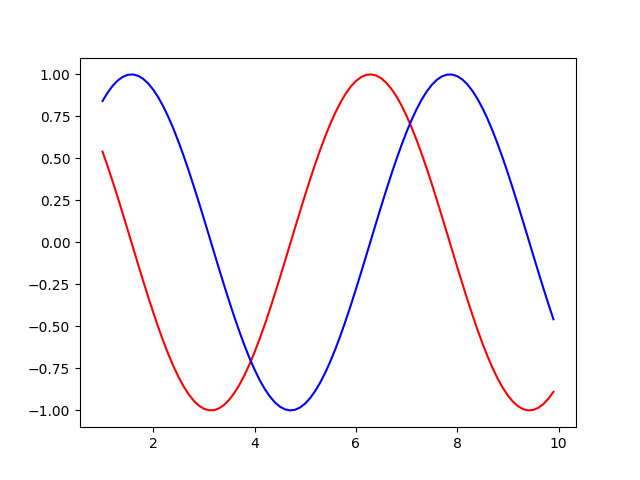
\includegraphics[width=.9\linewidth]{fig1.png}
\end{center}

\begin{minted}[,frame=single, framesep=10pt, linenos]{python}

over = [1,2,3,4,5]
run = [13,5,7,16,4]
plt.xlabel("Overs")
plt.ylabel("Runs")
plt.plot(over, run, 'r', marker='d', markersize=6, markeredgecolor='red')

\end{minted}

\begin{center}
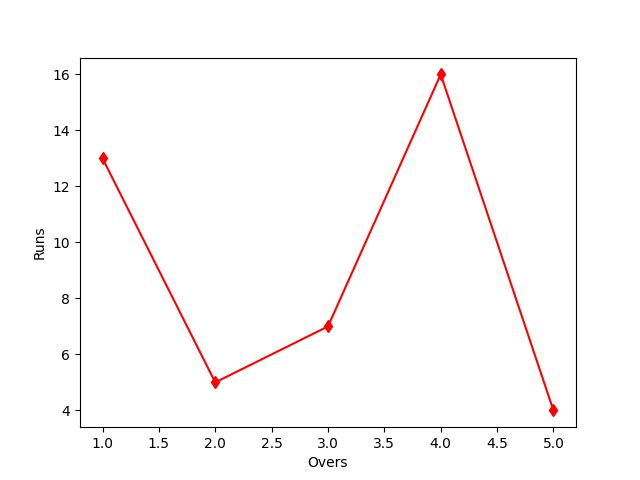
\includegraphics[width=.9\linewidth]{fig2.png}
\end{center}

\begin{minted}[,frame=single, framesep=10pt, linenos]{python}

over = [1,2,3,4,5]
run = [13,5,7,16,4]
plt.xlabel("Overs")
plt.ylabel("Runs")
plt.bar(over, run, width=1/2, color = ['r', 'g', 'b', 'k', 'c'])
plt.show()

\end{minted}

\begin{center}
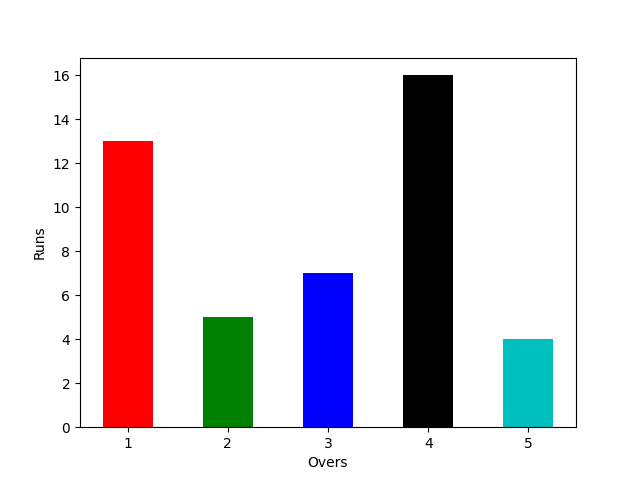
\includegraphics[width=.9\linewidth]{fig3.png}
\end{center}

\begin{minted}[,frame=single, framesep=10pt, linenos]{python}

over = np.arange(1.0,6.0,1.0)
ind = [13,5,7,16,14]
nz = [3,5,4,8,11]
plt.xlabel("Overs")
plt.ylabel("Runs")
plt.xlim(0,6)
plt.title("Cricket Analysis")
plt.bar(over, ind, color='b', width=0.25, label = 'IND')
plt.bar(over+0.25, nz, color='r', width=0.25, label = 'NZ')
plt.legend(loc='upper left')

\end{minted}

\begin{center}
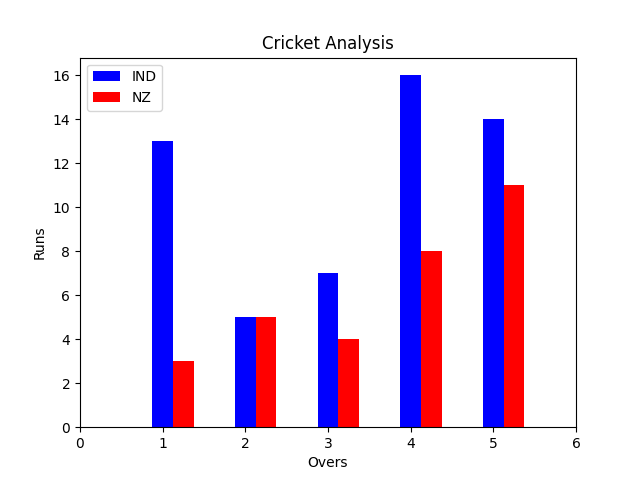
\includegraphics[width=.9\linewidth]{fig4.png}
\end{center}

\begin{minted}[,frame=single, framesep=10pt, linenos]{python}

proglang=['Python', 'C++', 'Java', 'Perl', 'Lisp']
performance=[10,7,6,4,2]
plt.xlabel=('Programming Languages')
plt.ylabel=('Performance')
plt.bar(proglang,performance, color='red')

\end{minted}

\begin{center}
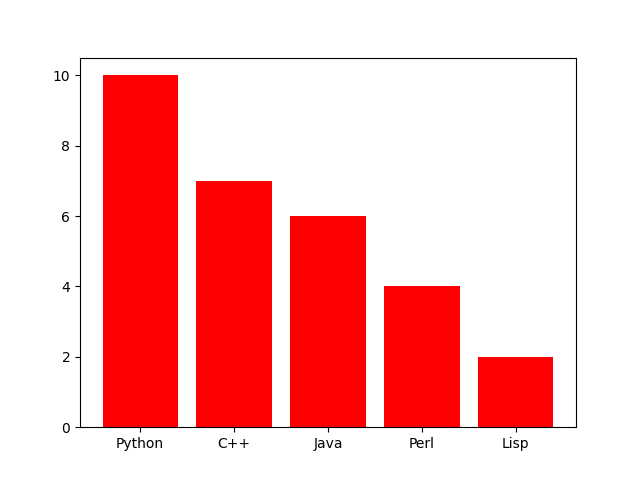
\includegraphics[width=.9\linewidth]{fig5.png}
\end{center}

\begin{minted}[,frame=single, framesep=10pt, linenos]{python}

import pandas as pd
x = {'speed':[10,15,20,18,19],\
        'meters':[122,150,190,230,300],\
         'weight':[0.2,0.3,0.1,0.85,0.0]}
df=pd.DataFrame(x)
plt.scatter(list(df['meters']), list(df['speed']))

\end{minted}

\begin{center}
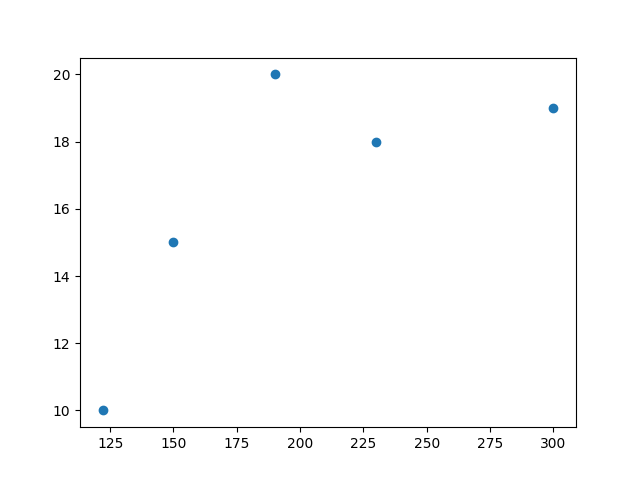
\includegraphics[width=.9\linewidth]{fig6.png}
\end{center}

\begin{minted}[,frame=single, framesep=10pt, linenos]{python}

import pandas as pd
x = {'speed':[10,15,20,18,19],\
        'meters':[122,150,190,230,300],\
         'weight':[0.2,0.3,0.1,0.85,0.0]}
df=pd.DataFrame(x)
plt.scatter(list(df['meters']), list(df['weight']))

\end{minted}

\begin{center}
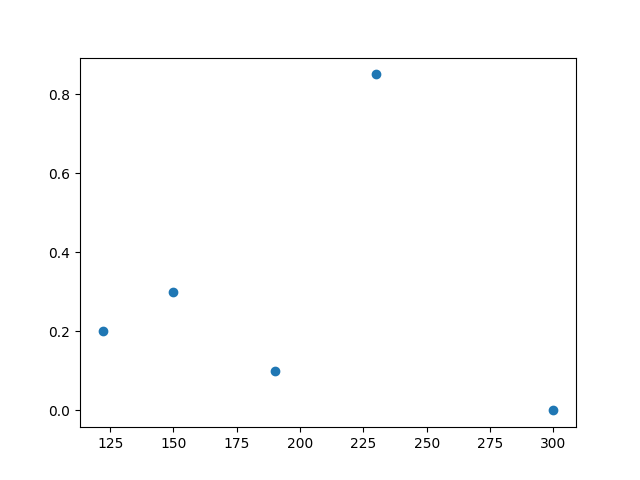
\includegraphics[width=.9\linewidth]{fig7.png}
\end{center}

\begin{minted}[,frame=single, framesep=10pt, linenos]{python}

import pandas as pd
df1 = pd.DataFrame({'1990':[52,64,78,94], '2000':[340,480,688,766], '2010':[890,560,1102,889]})
df1.index=['a', 'b', 'c', 'd']

plt.scatter(list(df1['1990']), list(df1['2000']))
plt.plot(df1['1990'], df1['2000'])


\end{minted}

\begin{center}
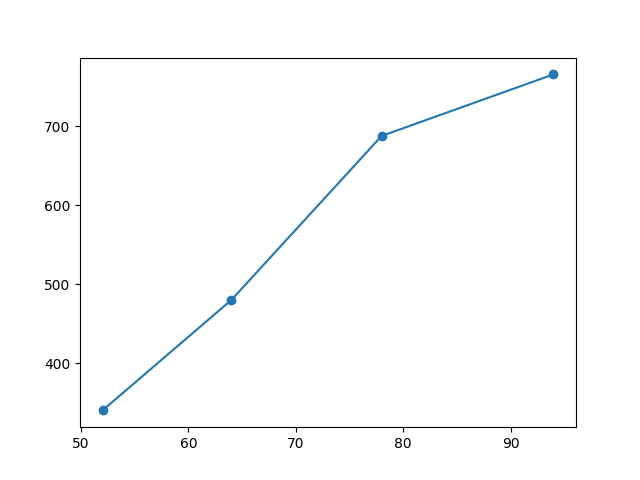
\includegraphics[width=.9\linewidth]{fig8.png}
\end{center}

\begin{minted}[,frame=single, framesep=10pt, linenos]{python}

import pandas as pd
df1 = pd.DataFrame({'1990':[52,64,78,94], '2000':[340,480,688,766], '2010':[890,560,1102,889]})
df1.index=['a', 'b', 'c', 'd']

plt.plot(df1['1990'], df1['2000'])


\end{minted}

\begin{center}
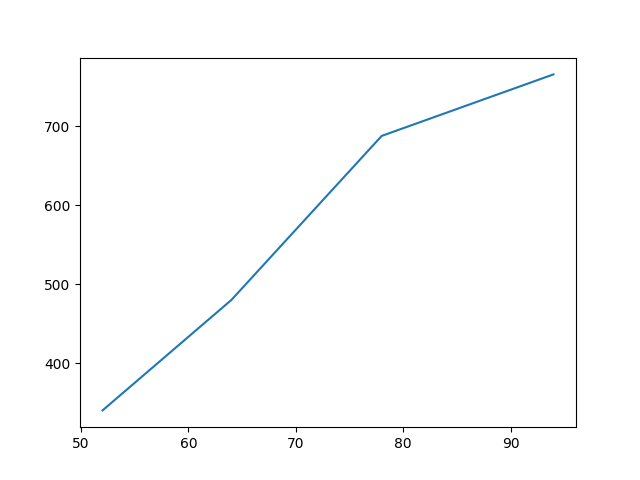
\includegraphics[width=.9\linewidth]{fig9.png}
\end{center}

\begin{minted}[,frame=single, framesep=10pt, linenos]{python}

import pandas as pd
df1 = pd.DataFrame({'1990':[52,64,78,94], '2000':[340,480,688,766], '2010':[890,560,1102,889]})
df1.index=['a', 'b', 'c', 'd']

df1.plot.bar()

\end{minted}

\begin{center}
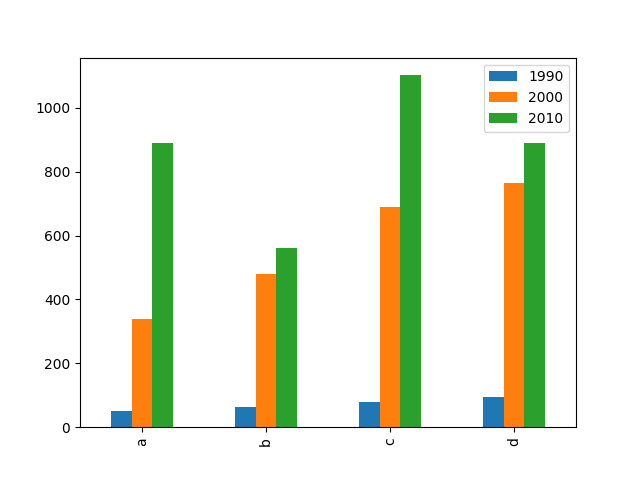
\includegraphics[width=.9\linewidth]{fig10.png}
\end{center}

\begin{minted}[,frame=single, framesep=10pt, linenos]{python}

import pandas as pd
df1 = pd.DataFrame({'Jan':[140, 160, 140, 180, 110], 'Feb':[130, 200, 180, 150, 160], 'Mar':[130, 130, 150, 200, 130], 'Apr':[190, 200, 170, 120, 110], 'May':[160, 200, 190, 180, 120], 'Jun':[200, 170, 140, 140, 170], 'Jul':[150, 110, 170, 110, 130], 'Aug':[170, 160, 180, 130, 200], 'Sep':[190, 130, 190, 150, 150], 'Oct':[170, 140, 150, 190, 160], 'Nov':[150, 170, 140, 110, 170], 'Dec':[120, 200, 170, 140, 130]})
df1.index=['North', 'South', 'East', 'West', 'Central']
print(df1)
df1.plot.bar()

\end{minted}

\begin{center}
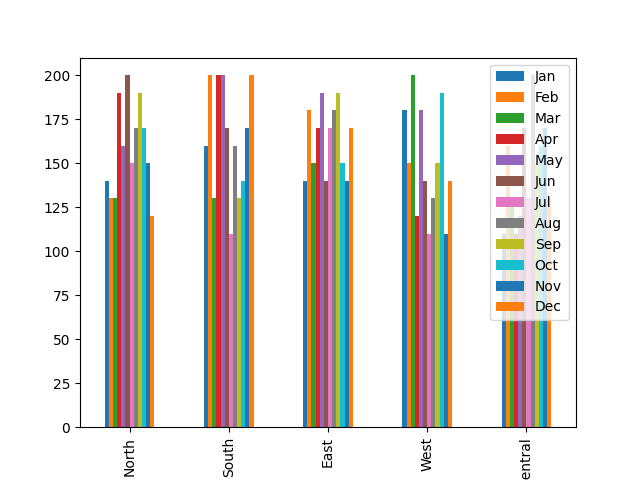
\includegraphics[width=.9\linewidth]{fig11.png}
\end{center}

\begin{minted}[,frame=single, framesep=10pt, linenos]{python}

import pandas as pd
df1 = pd.DataFrame({'Jan':[140, 160, 140, 180, 110], 'Feb':[130, 200, 180, 150, 160], 'Mar':[130, 130, 150, 200, 130], 'Apr':[190, 200, 170, 120, 110], 'May':[160, 200, 190, 180, 120], 'Jun':[200, 170, 140, 140, 170], 'Jul':[150, 110, 170, 110, 130], 'Aug':[170, 160, 180, 130, 200], 'Sep':[190, 130, 190, 150, 150], 'Oct':[170, 140, 150, 190, 160], 'Nov':[150, 170, 140, 110, 170], 'Dec':[120, 200, 170, 140, 130]})
df1.index=['North', 'South', 'East', 'West', 'Central']
plt.plot(df1.columns.values.tolist(), df1.loc['North',:], label='North')
plt.plot(df1.columns.values.tolist(), df1.loc['South',:], label='South')
plt.plot(df1.columns.values.tolist(), df1.loc['East',:], label='East')
plt.plot(df1.columns.values.tolist(), df1.loc['West',:], label='West')
plt.plot(df1.columns.values.tolist(), df1.loc['Central',:], label='Central')
plt.legend()

\end{minted}

\begin{center}
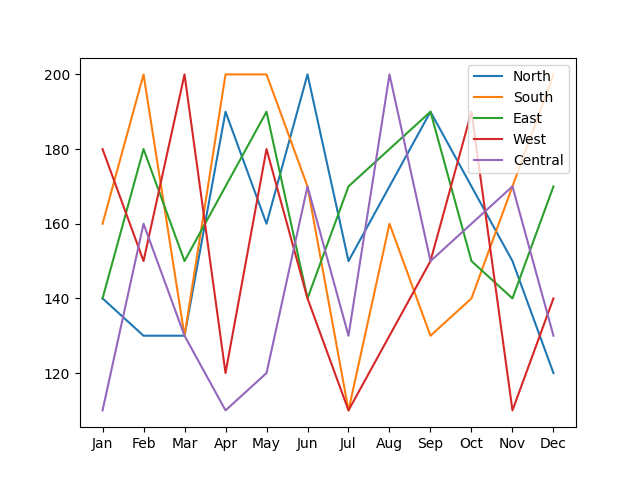
\includegraphics[width=.9\linewidth]{fig12.png}
\end{center}
\end{document}